\section{Results}\label{Sec:Results}

\subsection{Sample Preparation}

Before pooling the adaptor-ligated and indexed sequencing libraries, the sucess of
library preparation is validated using the Agilent Bioanalyzer instrument. \ref{fig:f1}
and \ref{fig:f2} show representative electropherograms of a sample that has been
processed using both kits. The expected DNA products should be detected at 175-600 bp
for Haloplex CSC and 200-400 for TST15.

\begin{figure}[!htbp]
  \centering
  \subfloat[Agilent Haloplex CSC (High Sensitivity DNA Chip)]{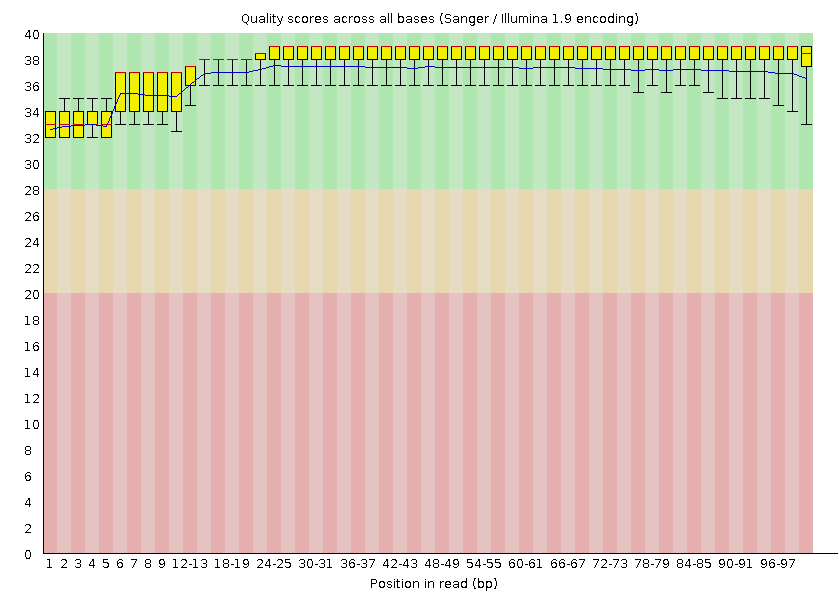
\includegraphics[width=0.45\textwidth]{fastq_halo_forward.png}\label{fig:f1}}
  \hfill
  \subfloat[Illumina TST15 (MixA) (DNA 1000 DNA Chip)]{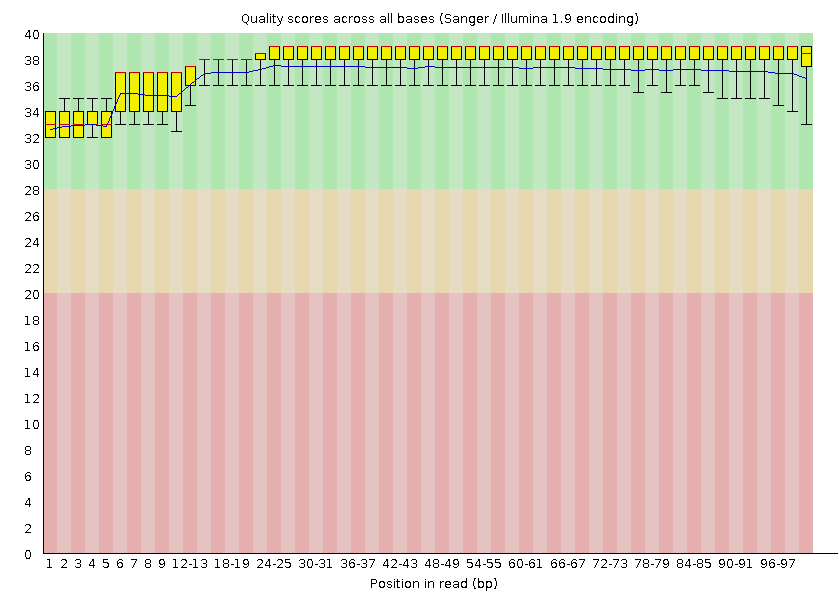
\includegraphics[width=0.45\textwidth]{fastq_halo_forward.png}\label{fig:f2}}
  \caption{Electropherograms of representative sequencing libraries prepared by Agilent Haloplex ClearSeq Cancer and Illumina TruSight Tumor 15. (*) represents the lower marker, (**) represents the upper marker}
\end{figure}

\begin{figure}[!htbp]
  \begin{center}
    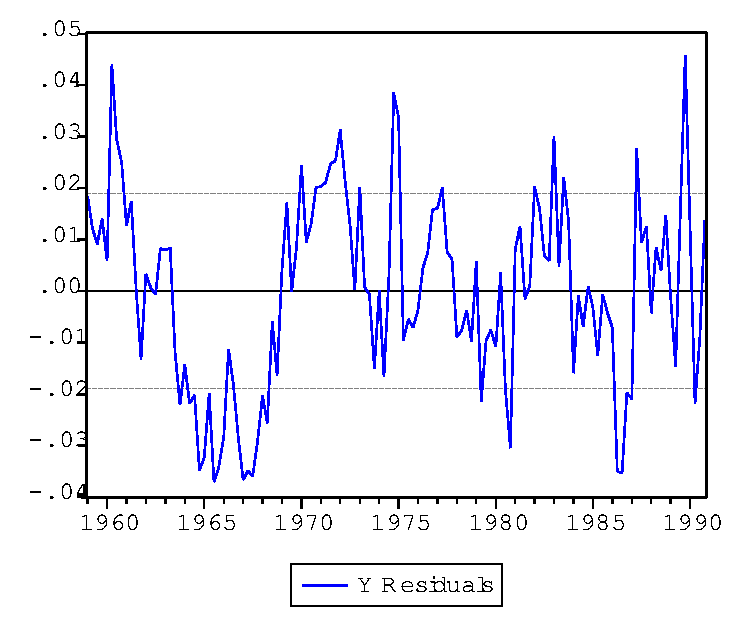
\includegraphics[scale=0.75,angle=0]{graph.pdf}
    \caption{Scatter plot of the corrected peak area (X axis) of the regions corresponding to the sequencing libraries defined in the blabla software and the dCt (Y axis). Agilent Haloplex ClearSeq Cancer data are represented as blue dots, Illumina TruSight Tumor 15 data are represented as red dots.}
    \label{Fig:bioanalyzer_scatter}
  \end{center}
\end{figure}

Using the blablabla software, the concentration, molarity and total peak area (TPA)
of the expected sequencing libraries were calculated.

Hopefully: there is a relationship between dCt and TPA. Maybe: Haloplex is more
affected by bad dCt values.

\subsection{NGS Data Quality}

Sequencing run parameters were calculated by the Illumina Sequencing Viewer software.
Table XXX shows the averaged run parameters of runs with Haloplex CSC and TST15
sample preparation.

\begin{table}[!htbp]
    \caption[ISV]{Comparison of Run Parameters (Averaged) of Sequencing Runs with Haloplex CSC \& TST15 Sample Preparation}
    \centering
    \begin{tabular}{ |p{4.5cm}|p{2cm}|p{2cm}|}
    \hline
    Parameter & Haloplex CSC & TST15 \\ \hline
    Yield total (Gb) & 3.7 & 7.37 \\
    \% \textgreater Q30 & 93.8 & 82.355 \\
    Cluster Density PF (k/mm2) & 1084 & 1180  \\
    Cluster Density PF (\%) & 85.95 & 79.95 \\
    \hline
    \label{sequencing_viewer}
  \end{tabular}
\end{table}

TST15 has a higher cluster density and therefore a higher total yield, but has
lower reads passing a phred-score threshold of Q30 than Haloplex. This is due to
the different chemistries used. TST15 uses v3 chemistry, while Haloplex uses v2.
v2 generally has lower cluster density and output, but therefore better quality.

\begin{figure}[!tbp]
  \centering
  \subfloat[Agilent Haloplex ClearSeq Cancer]{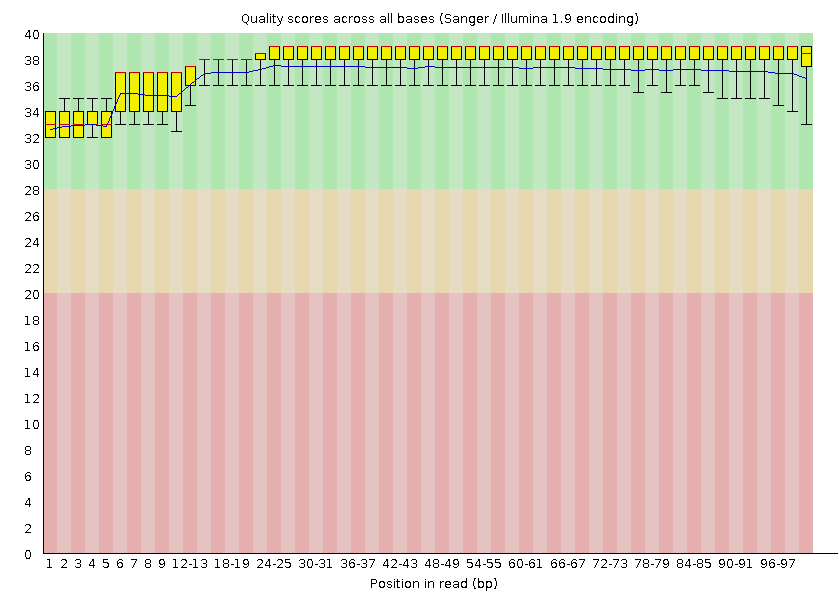
\includegraphics[width=0.5\textwidth]{fastq_halo_forward.png}\label{fig:amp_dist_hpx}}
  \hfill
  \subfloat[Illumina TruSight Tumor 15]{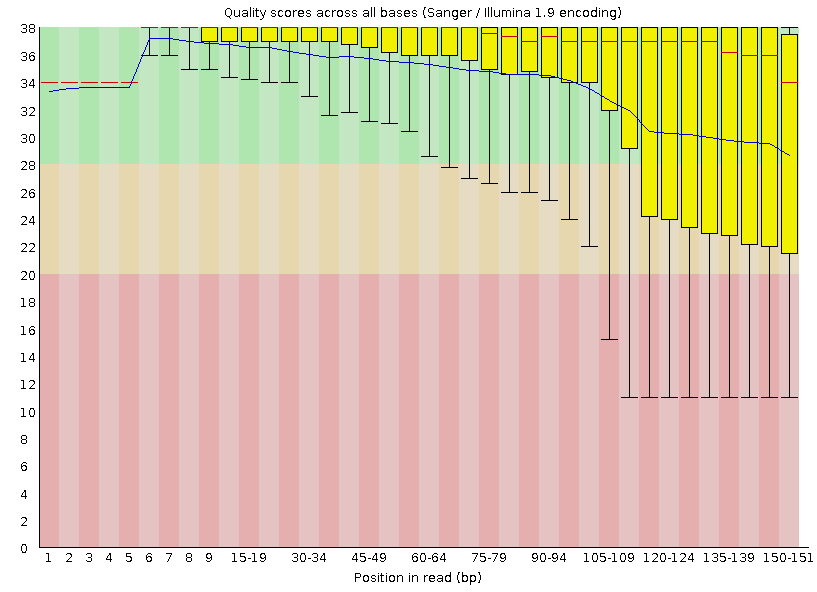
\includegraphics[width=0.5\textwidth]{fastq_tst15_forward.png}\label{fig:amp_dist_tst}}
  \caption{Comparison of coverage distributions per amplicon as reported by FastQC}
\end{figure}

Table XXX shows the boxplot representations of the read qualities per position
of two representative FASTQ files as reported by FastQC. Both workflows yield high
quality data, yet Haloplex CSC data have more narrow distributions and are of higher
quality. This is in direct relationship with the sequencing chemistry kit used.

\begin{table}
\begin{tabular}{p{3.5cm} p{1cm} p{1cm}}\\
\hline
Parameter & Haloplex CSC & TST15 \\
\hline
\% mapped & 91 & 62.6 \\
\% paired & 0 & 58.7 \\
\% singletons & 1.8 & 3.8 \\
\label{samtools_flagstat}
\end{tabular}
\end{table}

The Samtools Flagstat command was used to determine some basic BAM statistics of BAM
files of samples prepared with the respective library preparations and processed with
the mentioned bioinformatic pipelines. \ref{table:samtools_flagstat} shows the
averaged result of these statistics.

Considering the recommended pipelines, Haloplex
CSC data, analyzed with Agilent's SureCall software, has a higher percentage (91\%) of mapped
reads when compared to Illumina's BaseSpace TruSight Tumor 15 App (62.9\%). Data analysis
with the recommended SureCall design includes a steps where mates are fixed, but they
are not stitched together. Therefore no reads are considered as being paired. The TST15 app
in contrast includes a read stitching step and 58\% are considered as properly paired.
This means that of the 62.6\% of mapped reads, 4.2\% are not properly paired. 3.8\%
of reads processed with the TST15 online App are considered to be singletons, whereas
only 1.8\% of reads processed with the SureCall software are considered as singletons.

\subsection{Coverage Analysis}

Coverage Distribution TST15 vs Haloplex

Coverage Distribution per Patient (check if correlation IQR with dCt)

Coverage Distribution per Amplicon (check if some have always lower coverage, check if some failed)
\begin{figure}[!tbp]
  \centering
  \subfloat[Agilent Haloplex ClearSeq Cancer]{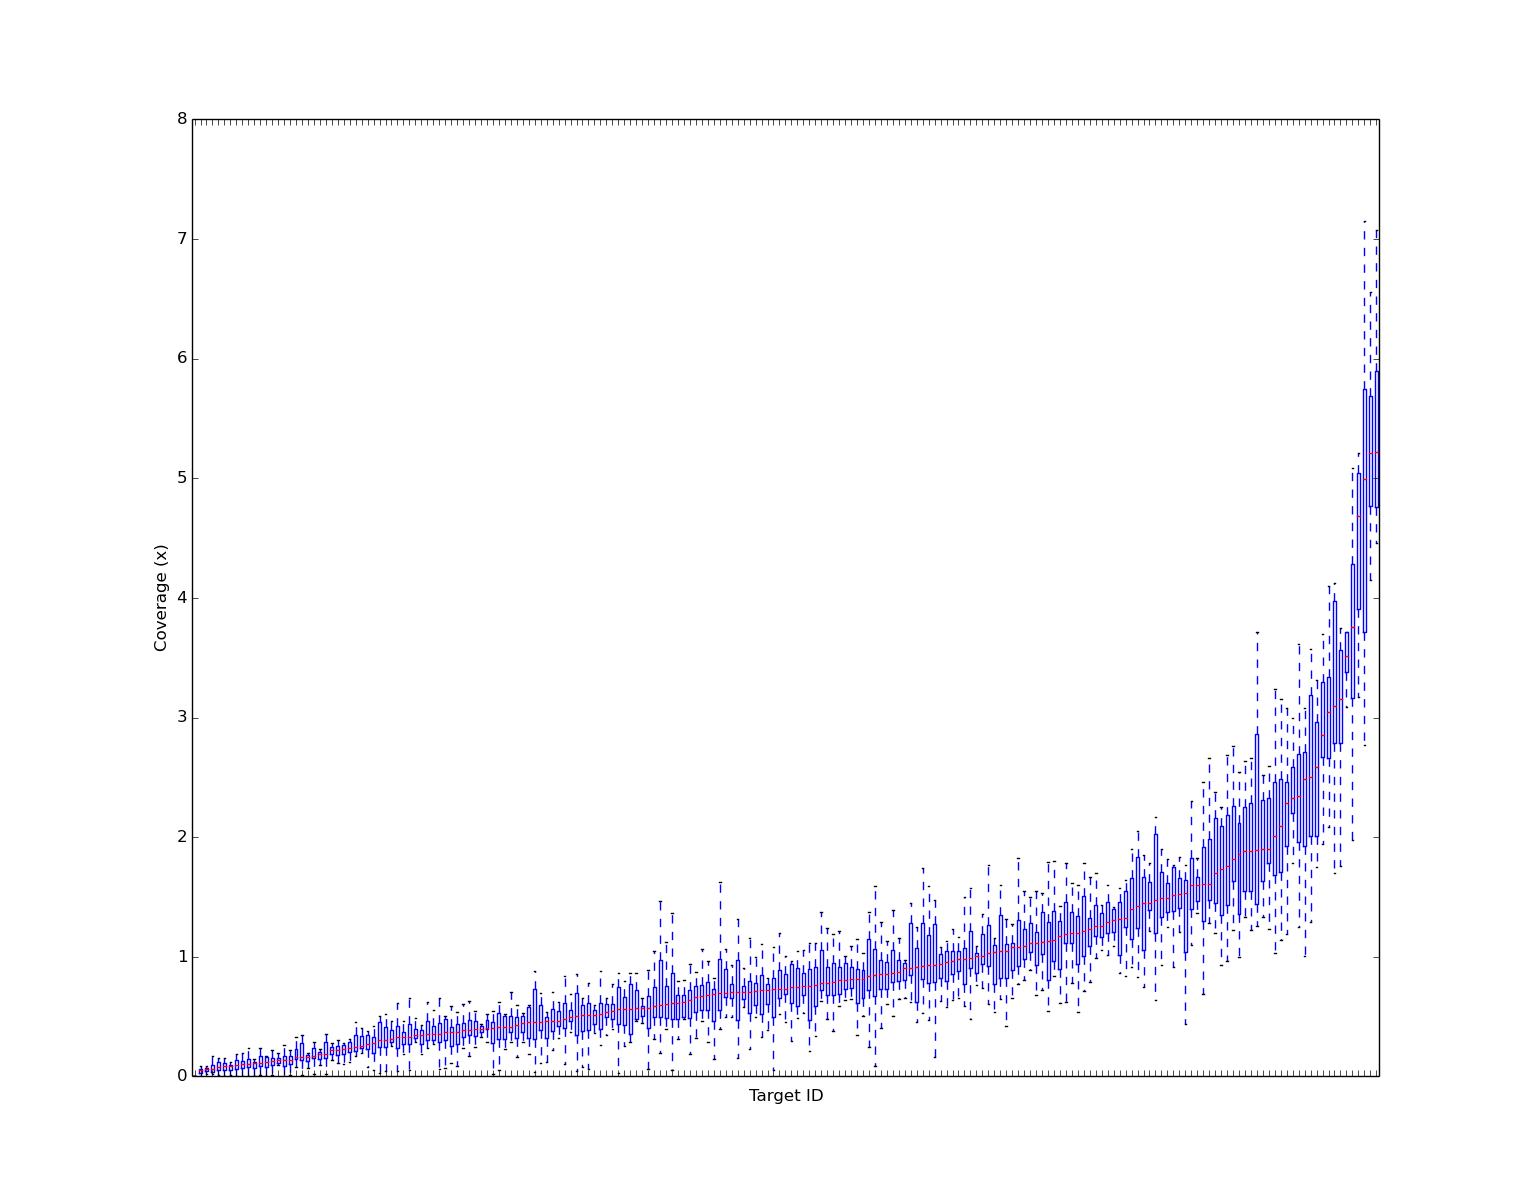
\includegraphics[width=0.5\textwidth]{distribution_amplicons_hap_csc.png}\label{fig:amp_dist_hpx}}
  \hfill
  \subfloat[Illumina TruSight Tumor 15]{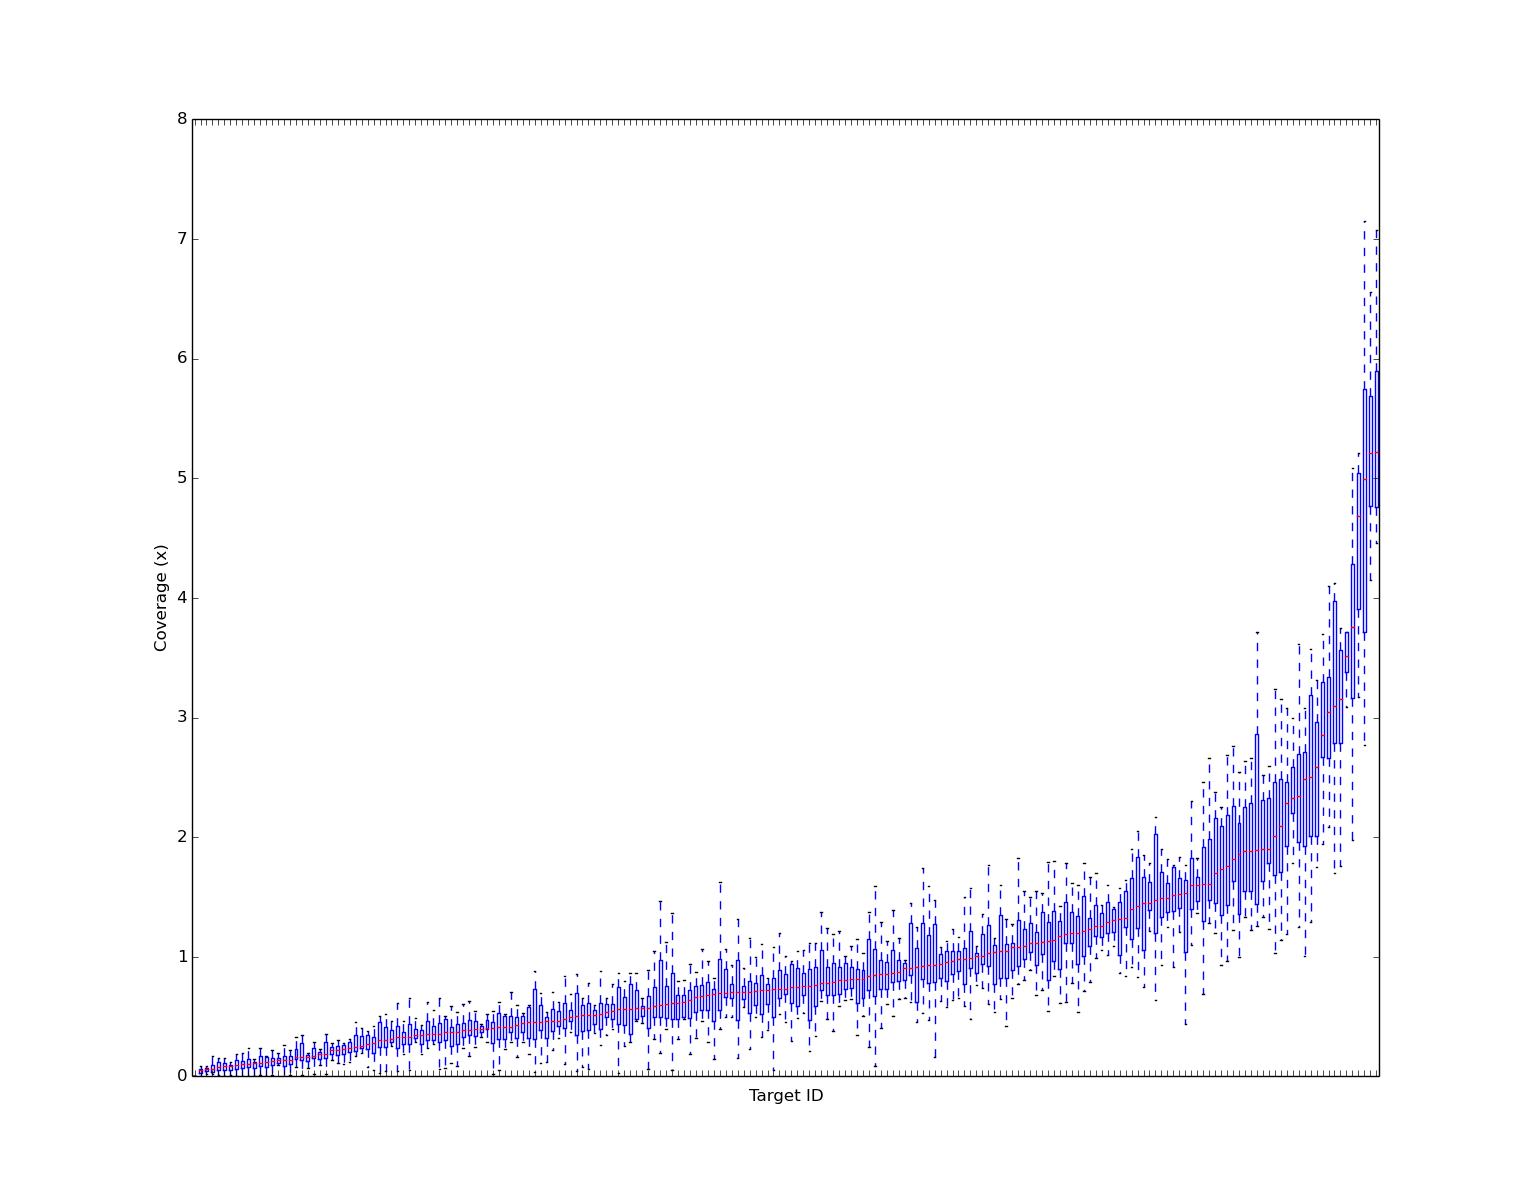
\includegraphics[width=0.5\textwidth]{distribution_amplicons_hap_csc.png}\label{fig:amp_dist_tst}}
  \caption{Comparison of Coverage Distributions per Amplicon}
\end{figure}

% Merge TST15 MixA & MixB together in one figure.
% Try to extract median values out of boxplots; new figure with these points
% -> some kind of trend line. The sooner it gets to a normalized coverage value of 1,
% the better.

% Looks like TST15 are better than Haloplex. But problem in TST: some EGFR & KRAS
% have low distributions.

% Do the same for EGFR; KRAS; NRAS; BRAF

Failed Amplicon Counter

\begin{minipage}{0.5\textwidth}
\captionof{table}{Failed Amplicons in Agilent Haloplex ClearSeq Cancer}
\begin{tabular}{p{1.5cm} p{1.5cm} p{1.5cm}}\\
\hline
Amplicon & Coverage Failed & No of Samples \\
\hline
ATM_14 & 1 & all \\
Bla & 200 & 9 \\
Blabla & 500 & 5 \\
\label{failed_hpx}
\end{tabular}
\end{minipage}
\hfill
\begin{minipage}{0.5\textwidth}
\captionof{table}{Failed Amplicons in Illumina TruSight Tumor 15}
\begin{tabular}{p{3cm} p{1.5cm} p{1.5cm}}\\
\hline
Amplicon & Coverage Failed & No of Samples \\
\hline
ATM_14 & 1 & all \\
Bla & 200 & 9 \\
Blabla & 500 & 5 \\
\label{failed_tst}
\end{tabular}
\end{minipage}

Fragmentation <-> Coverage?
% Scatter plot: dCt vs normalized coverage (median / IQR ???)

(GATK CallableLoci)
(GATK CountLoci???)
(GATK FindCoveredIntervals)

On-off target; Enrichment Efficiency TST15 vs Haloplex

Coverage across genome, check where there is coverage

Strandedness?

GATK DepthOfCoverage???

\subsection{Variant Calling Algorithm Comparison}
Detection of Known Single Nucleotide Variants and Deletions

Which should be found?

Which have not been found? Why?

MuTect

VarScan

GATK HaplotypeCaller

SomVarIUS????????
Freebayes????????
Vardict???????

SureCall & TST15

Tools that may be of use somehow: GATK SelectVariants; GATK VariantFiltration; GATK VariantEval; GATK ValidateVariants

More C>T ?
